\documentclass[10pt]{beamer}

\usetheme[progressbar=frametitle]{metropolis}
\usepackage{appendixnumberbeamer}

\usepackage{booktabs}
\usepackage[scale=2]{ccicons}

\usepackage{pgfplots}
\usepgfplotslibrary{dateplot}

\usepackage{xspace}
\newcommand{\themename}{\textbf{\textsc{metropolis}}\xspace}

% подключаем кириллицу 
\usepackage[T2A]{fontenc}
\usepackage[utf8]{inputenc}
\usepackage{listings}
\usepackage{graphicx}
\usepackage{hyperref}
\usepackage{chronology}


\title{Metropolis}
\subtitle{A modern beamer theme}
% \date{\today}
\date{}
\author{Matthias Vogelgesang}
\institute{Center for modern beamer themes}
% \titlegraphic{\hfill
\includegraphics[height=1.5cm]{logo.pdf}}





\title{Семинар 2}
\subtitle{Графы. Деревья.}
%\date{\small{\jobname}}
%\date{\today}
\author{\texttt{Бирюков Владимир}}
\institute{МФТИ}



\begin{document}

%-=-=-=-=-=-=-=-=-=-=-=-=-=-=-=-=-=-=-=-=-=-=-=-=
%
%	TITLE PAGE
%
%-=-=-=-=-=-=-=-=-=-=-=-=-=-=-=-=-=-=-=-=-=-=-=-=

\maketitle

%\begin{frame}[plain]
%	\titlepage
%\end{frame}

%-=-=-=-=-=-=-=-=-=-=-=-=-=-=-=-=-=-=-=-=-=-=-=-=
%
%	TABLE OF CONTENTS: OVERVIEW
%
%-=-=-=-=-=-=-=-=-=-=-=-=-=-=-=-=-=-=-=-=-=-=-=-=

\section{Введение в теорию графов}

%-=-=-=-=-=-=-=-=-=-=-=-=-=-=-=-=-=-=-=-=-=-=-=-=
%	TM: AT and definition
%-=-=-=-=-=-=-=-=-=-=-=-=-=-=-=-=-=-=-=-=-=-=-=-=


\begin{frame}{Граф}
\begin{columns}
\begin{column}{.48\linewidth}
Граф -- это математический объект, совокупность:
\begin{itemize}
\item $V$ = вершины
\item $E$ = ребра
\end{itemize}
Обозначается как $G = (V, E)$ \\
$n = |V|$ -- число вершин
$m = |E|$ -- число рёбер
\end{column}
\begin{column}{.48\linewidth}
		\begin{figure}
		\centerline{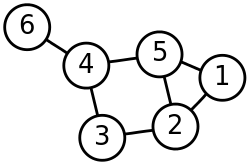
\includegraphics[width=1.0\linewidth]{images/graph1.png}}
		\end{figure}
	\end{column}
\end{columns}
\end{frame}



\begin{frame}{Граф}
\begin{enumerate}
\item связный граф -- если для любых вершин u,v есть путь из u в v.
\item взвешенный граф -- если каждому ребру графа поставлено в соответствие некоторое число, называемое весом ребра.
\item простой граф -- если он не имеет петель и кратных рёбер.
\item ациклический граф -- если он не имеет циклов.
\item дерево -- если он связный и ациклический.
\end{enumerate}
\begin{columns}
	\begin{column}{.3\linewidth}
		Ориентированный
		\begin{figure}
		\centerline{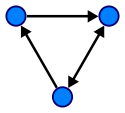
\includegraphics[width=1.0\linewidth]{images/und_graph.png}}
		\end{figure}
	\end{column}
	\begin{column}{.3\linewidth}
		Неориентированный
		\begin{figure}
		\centerline{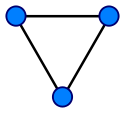
\includegraphics[width=1.0\linewidth]{images/d_graph.png}}
		\end{figure}
	\end{column}
\end{columns}
\end{frame}

\begin{frame}{Граф. Представления. Список смежных вершин. Матрица смежности.}
\begin{figure}
\centerline{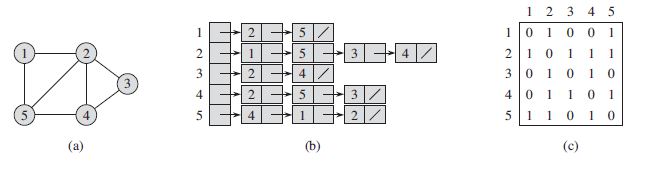
\includegraphics[width=1.1\linewidth]{images/graphrep1.png}}
\end{figure}
\end{frame}

\begin{frame}{Граф. Представления. Список смежных вершин. Матрица смежности.}
\begin{figure}
\centerline{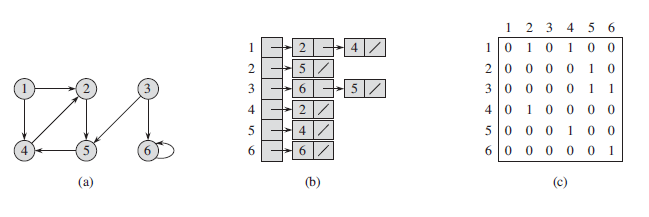
\includegraphics[width=1.1\linewidth]{images/graph_rep2.png}}
\end{figure}
\end{frame}



\begin{frame}{Граф}
\begin{columns}
	\begin{column}{.4\linewidth}
		Поиск в ширину
		\begin{figure}
		\centerline{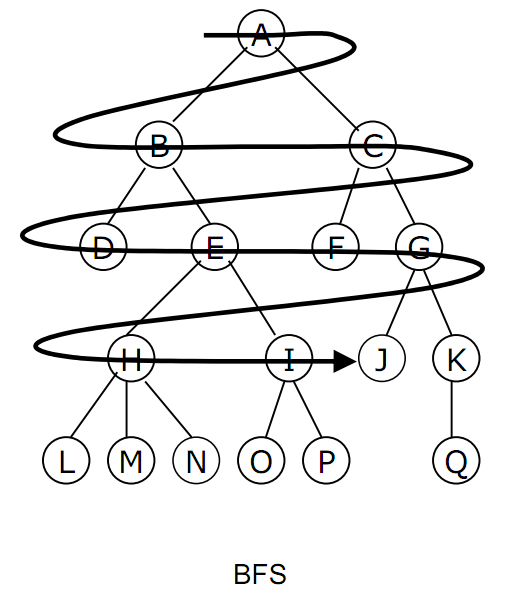
\includegraphics[width=1.0\linewidth]{images/bfs.png}}
		\end{figure}
	\end{column}
	\begin{column}{.4\linewidth}
		Поиск в глубину
		\begin{figure}
		\centerline{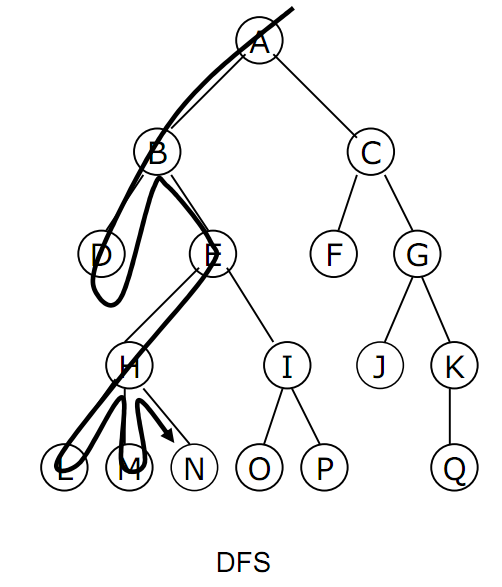
\includegraphics[width=1.0\linewidth]{images/dfs.png}}
		\end{figure}
	\end{column}
\end{columns}
\end{frame}


\begin{frame}{Граф. Псевдокод алгортма для BFS.}
\begin{figure}
\centerline{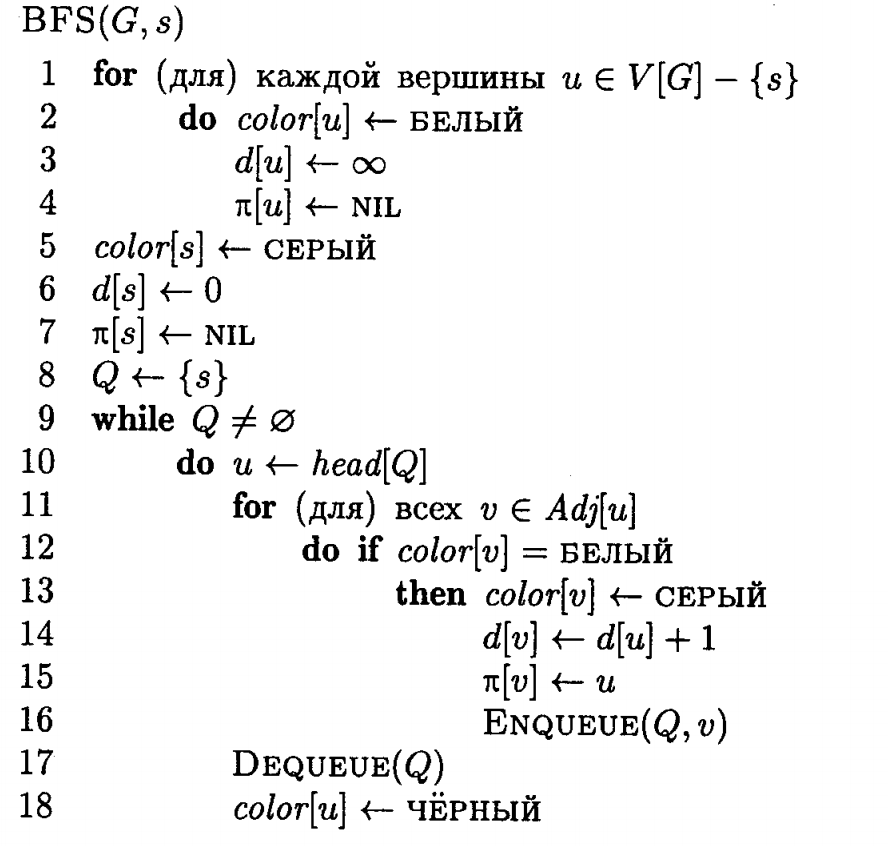
\includegraphics[width=0.7\linewidth]{images/bfs_algo.png}}
\end{figure}
\end{frame}

\begin{frame}{Граф. Алгортм BFS.}
\begin{figure}
\centerline{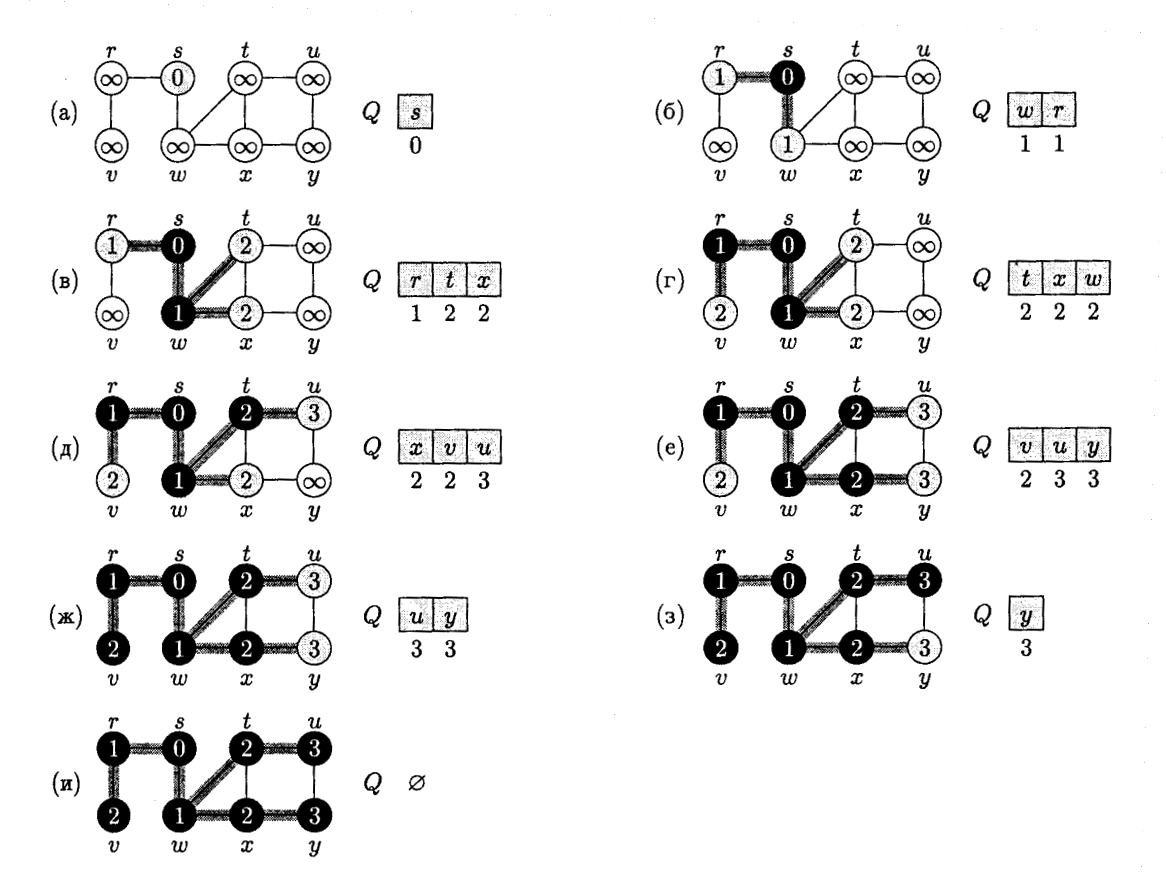
\includegraphics[width=1.0\linewidth]{images/bfs_graph.png}}
\end{figure}
\end{frame}



\begin{frame}{Очередь с приоритетом.}
\begin{figure}
\begin{itemize}
\item Абстрактный тип данных в программировании, поддерживающий две обязательные операции — добавить элемент и извлечь минимум.
\item Предполагается, что для каждого элемента можно вычислить его приоритет.
\item Простейшая реализация -- с помощью структуры данных куча(heap).
\item Асимптотическая сложность операций добавления и извлечения минимального в простейшей реализации -- $O(log(n))$.
\end{itemize}
\end{figure}
\end{frame}



\begin{frame}{Граф. Кратчайшие пути из одной вершины.}
\begin{figure}
\centerline{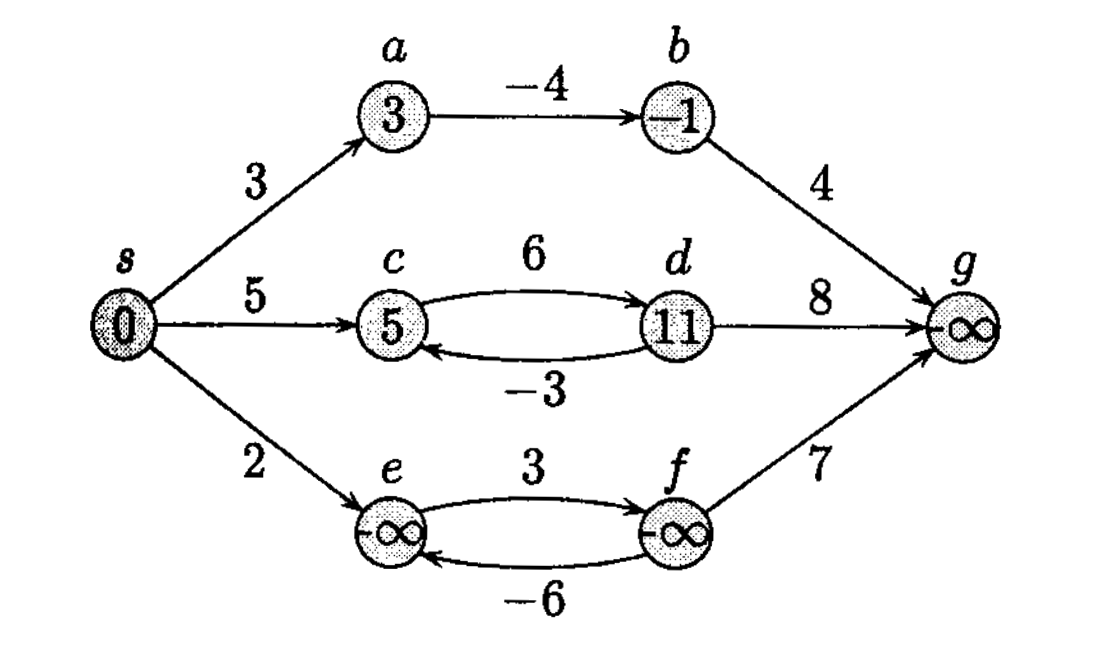
\includegraphics[width=1.0\linewidth]{images/closest1.png}}
\end{figure}
\end{frame}

\begin{frame}{Граф. Релаксация.}
\begin{figure}
\centerline{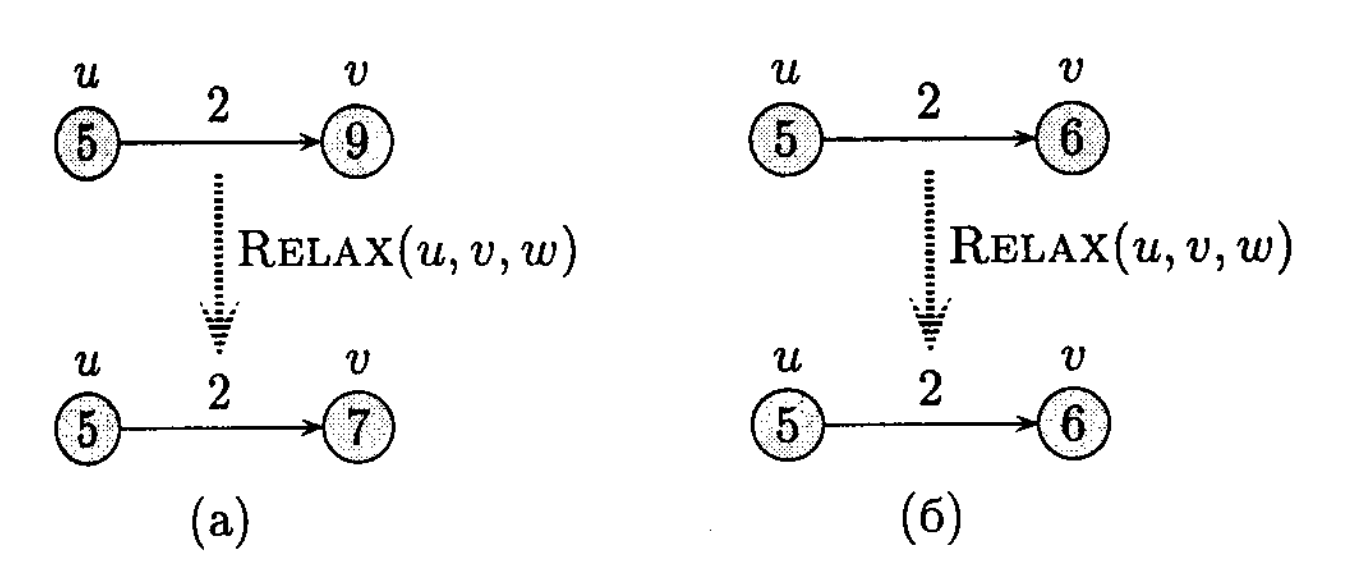
\includegraphics[width=1.0\linewidth]{images/relax.png}}
\end{figure}
\end{frame}

\begin{frame}{Граф. Алгоритм Дейкстры.}
\begin{figure}
\centerline{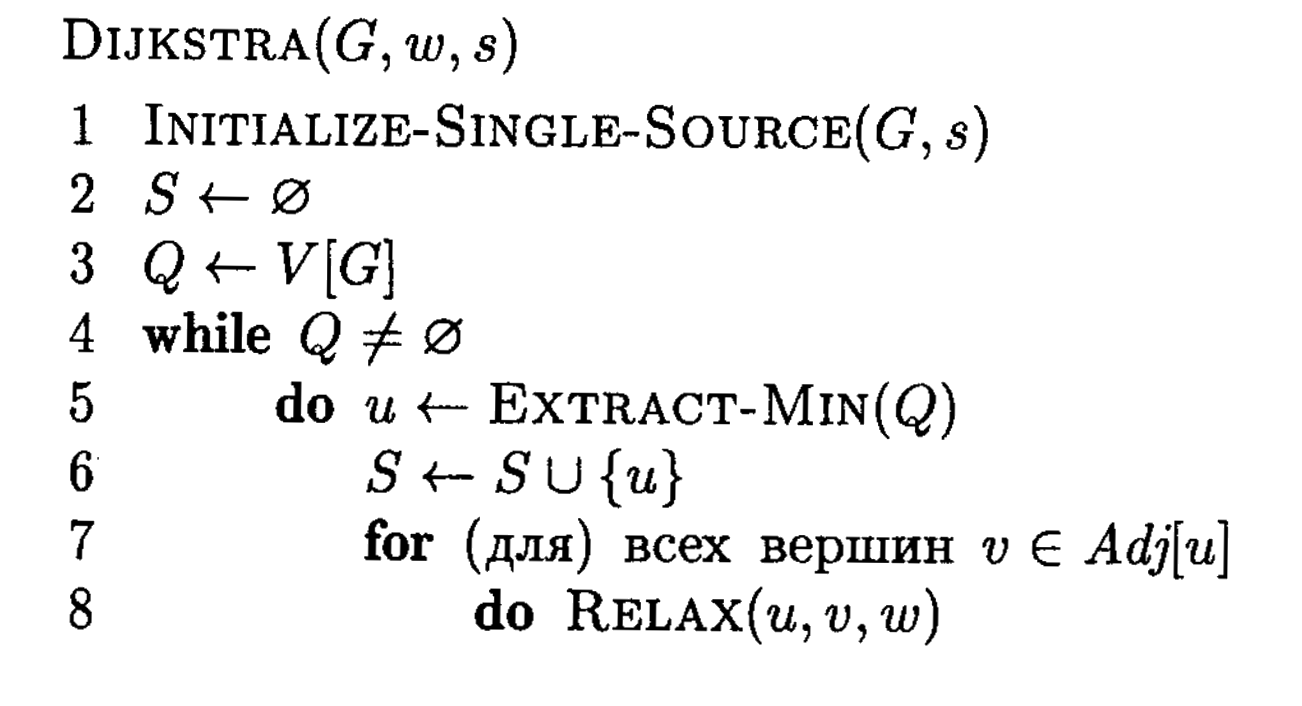
\includegraphics[width=1.0\linewidth]{images/deicstra_algo.png}}
\end{figure}
\end{frame}

\begin{frame}{Граф. Алгоритм Дейкстры.}
\begin{figure}
\centerline{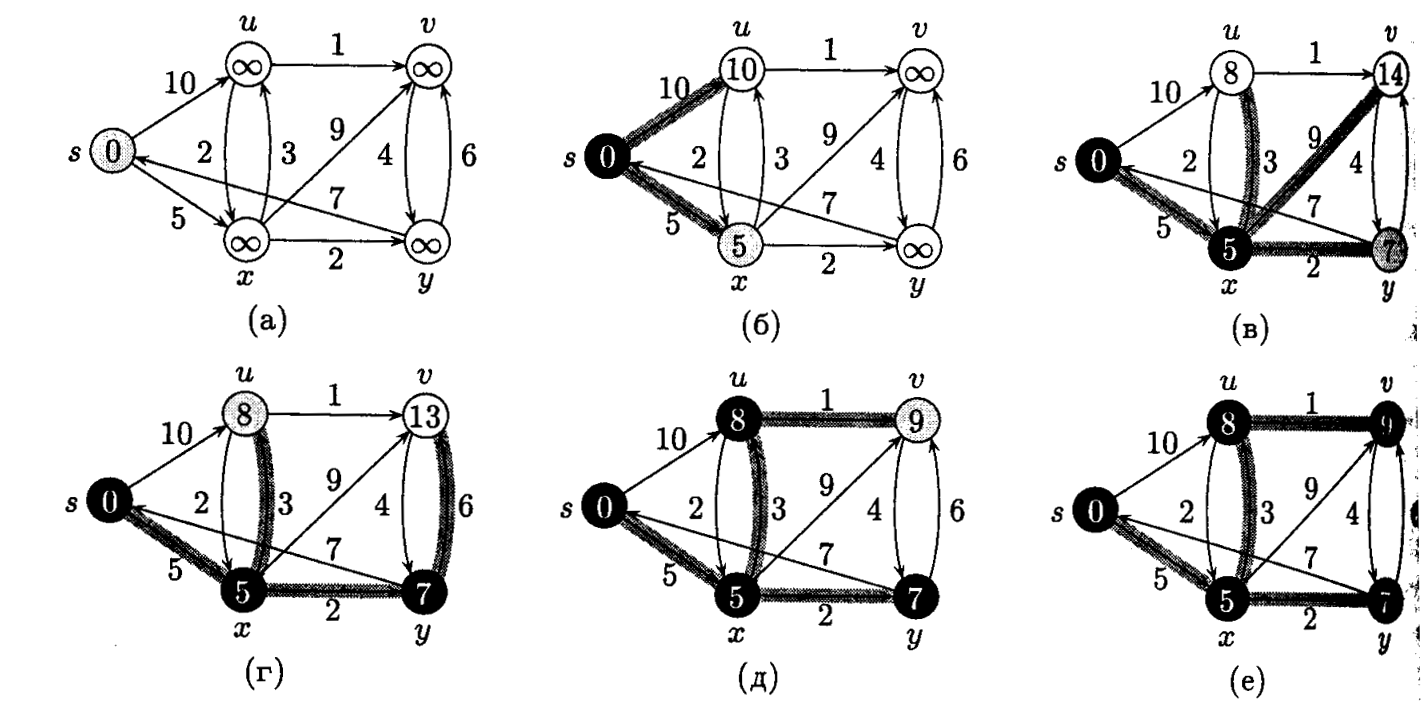
\includegraphics[width=1.0\linewidth]{images/deicstra_graphs.png}}
\end{figure}
\end{frame}



\begin{frame}{Граф. Сложности работы алгоритмов.}
\begin{itemize}
\item BFS -- $O(|V| + |E|)$
\item DFS -- $O(|V| + |E|)$
\item Алгоритм Дейкстры -- $O(|V|^2 + |E|)$
\item Алгоритм Беллмана-Форда -- $O(|V|*|E|)$ \\
(алгоритм нахождения кратчайших путей из одной вершины если есть отрицательные веса)
\item Алгоритм Флойда-Уоршолла -- $O(|V|^3)$ \\
(алгоритм нахождения кратчайших путей для всех пар вершин)
\end{itemize}
\end{frame}

%-=-=-=-=-=-=-=-=-=-=-=-=-=-=-=-=-=-=-=-=-=-=-=-=
%	Practical part:
%-=-=-=-=-=-=-=-=-=-=-=-=-=-=-=-=-=-=-=-=-=-=-=-=

\section{Деревья}

\begin{frame}{Деревья}
Дерево -- это связный граф без циклов.
\begin{columns}
	\begin{column}{.3\linewidth}
		\begin{figure}
		\centerline{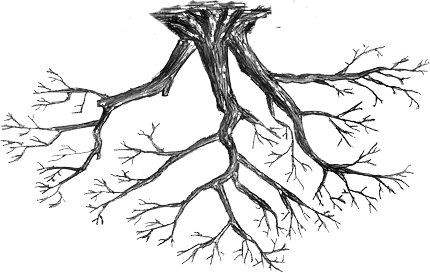
\includegraphics[width=1.6\linewidth]{images/littree.png}}
		\end{figure}
	\end{column}
	\begin{column}{.3\linewidth}
		\begin{figure}
		\centerline{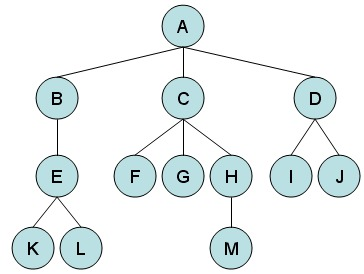
\includegraphics[width=1.6\linewidth]{images/tree.jpg}}
		\end{figure}
	\end{column}
\end{columns}
Двоичное дерево -- если у каждого узла не более двух потомков.
\end{frame}


\begin{frame}[fragile]
\frametitle{Двоичные деревья} 
\begin{center}
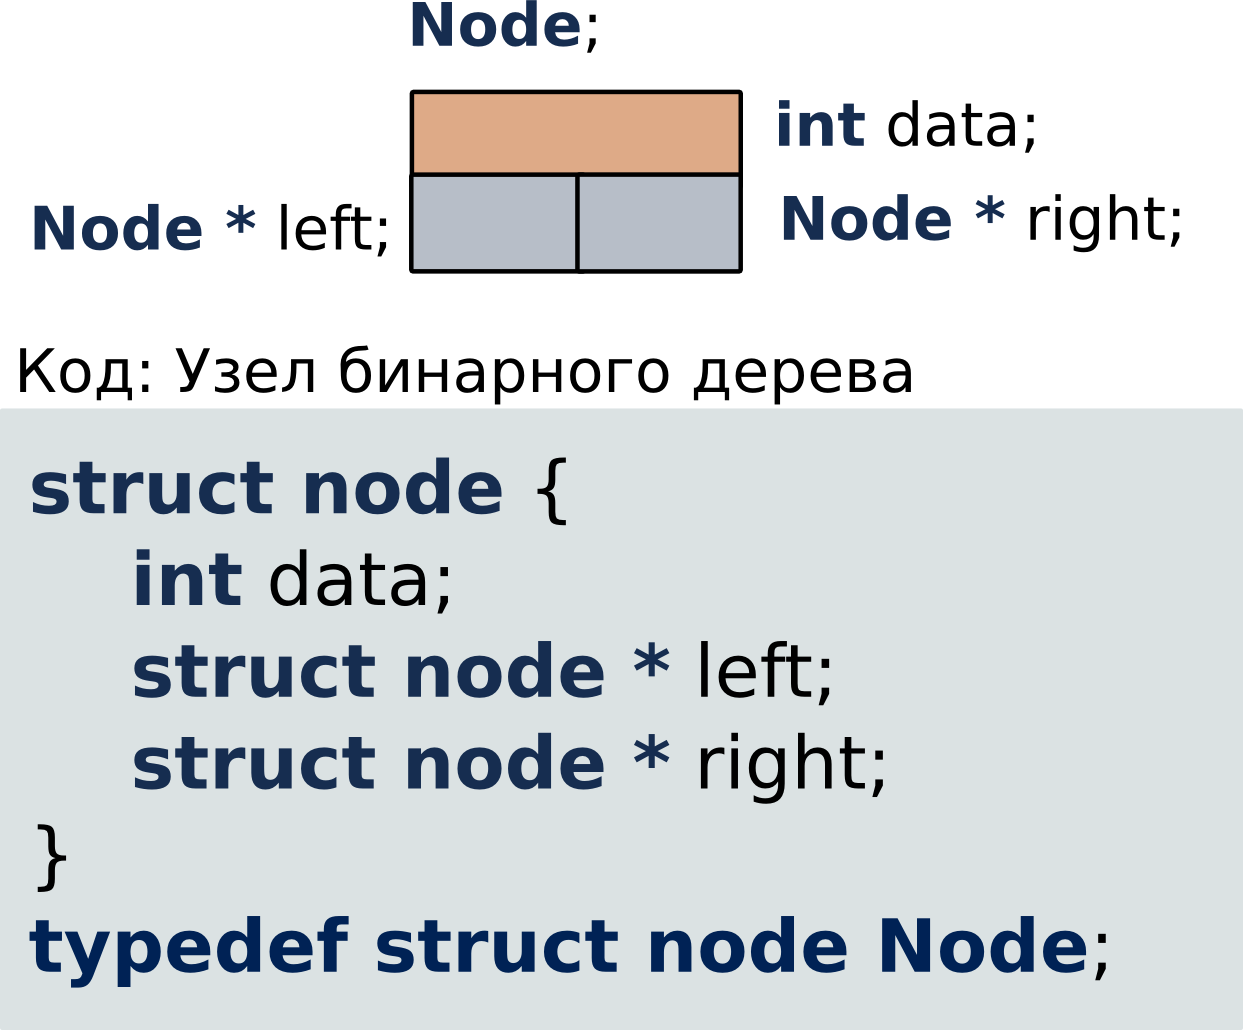
\includegraphics[width=0.6\linewidth]{images/bintree_initial.png}
\end{center}
\end{frame}
\begin{frame}[fragile]
\frametitle{Двоичные деревья}  
\begin{center}
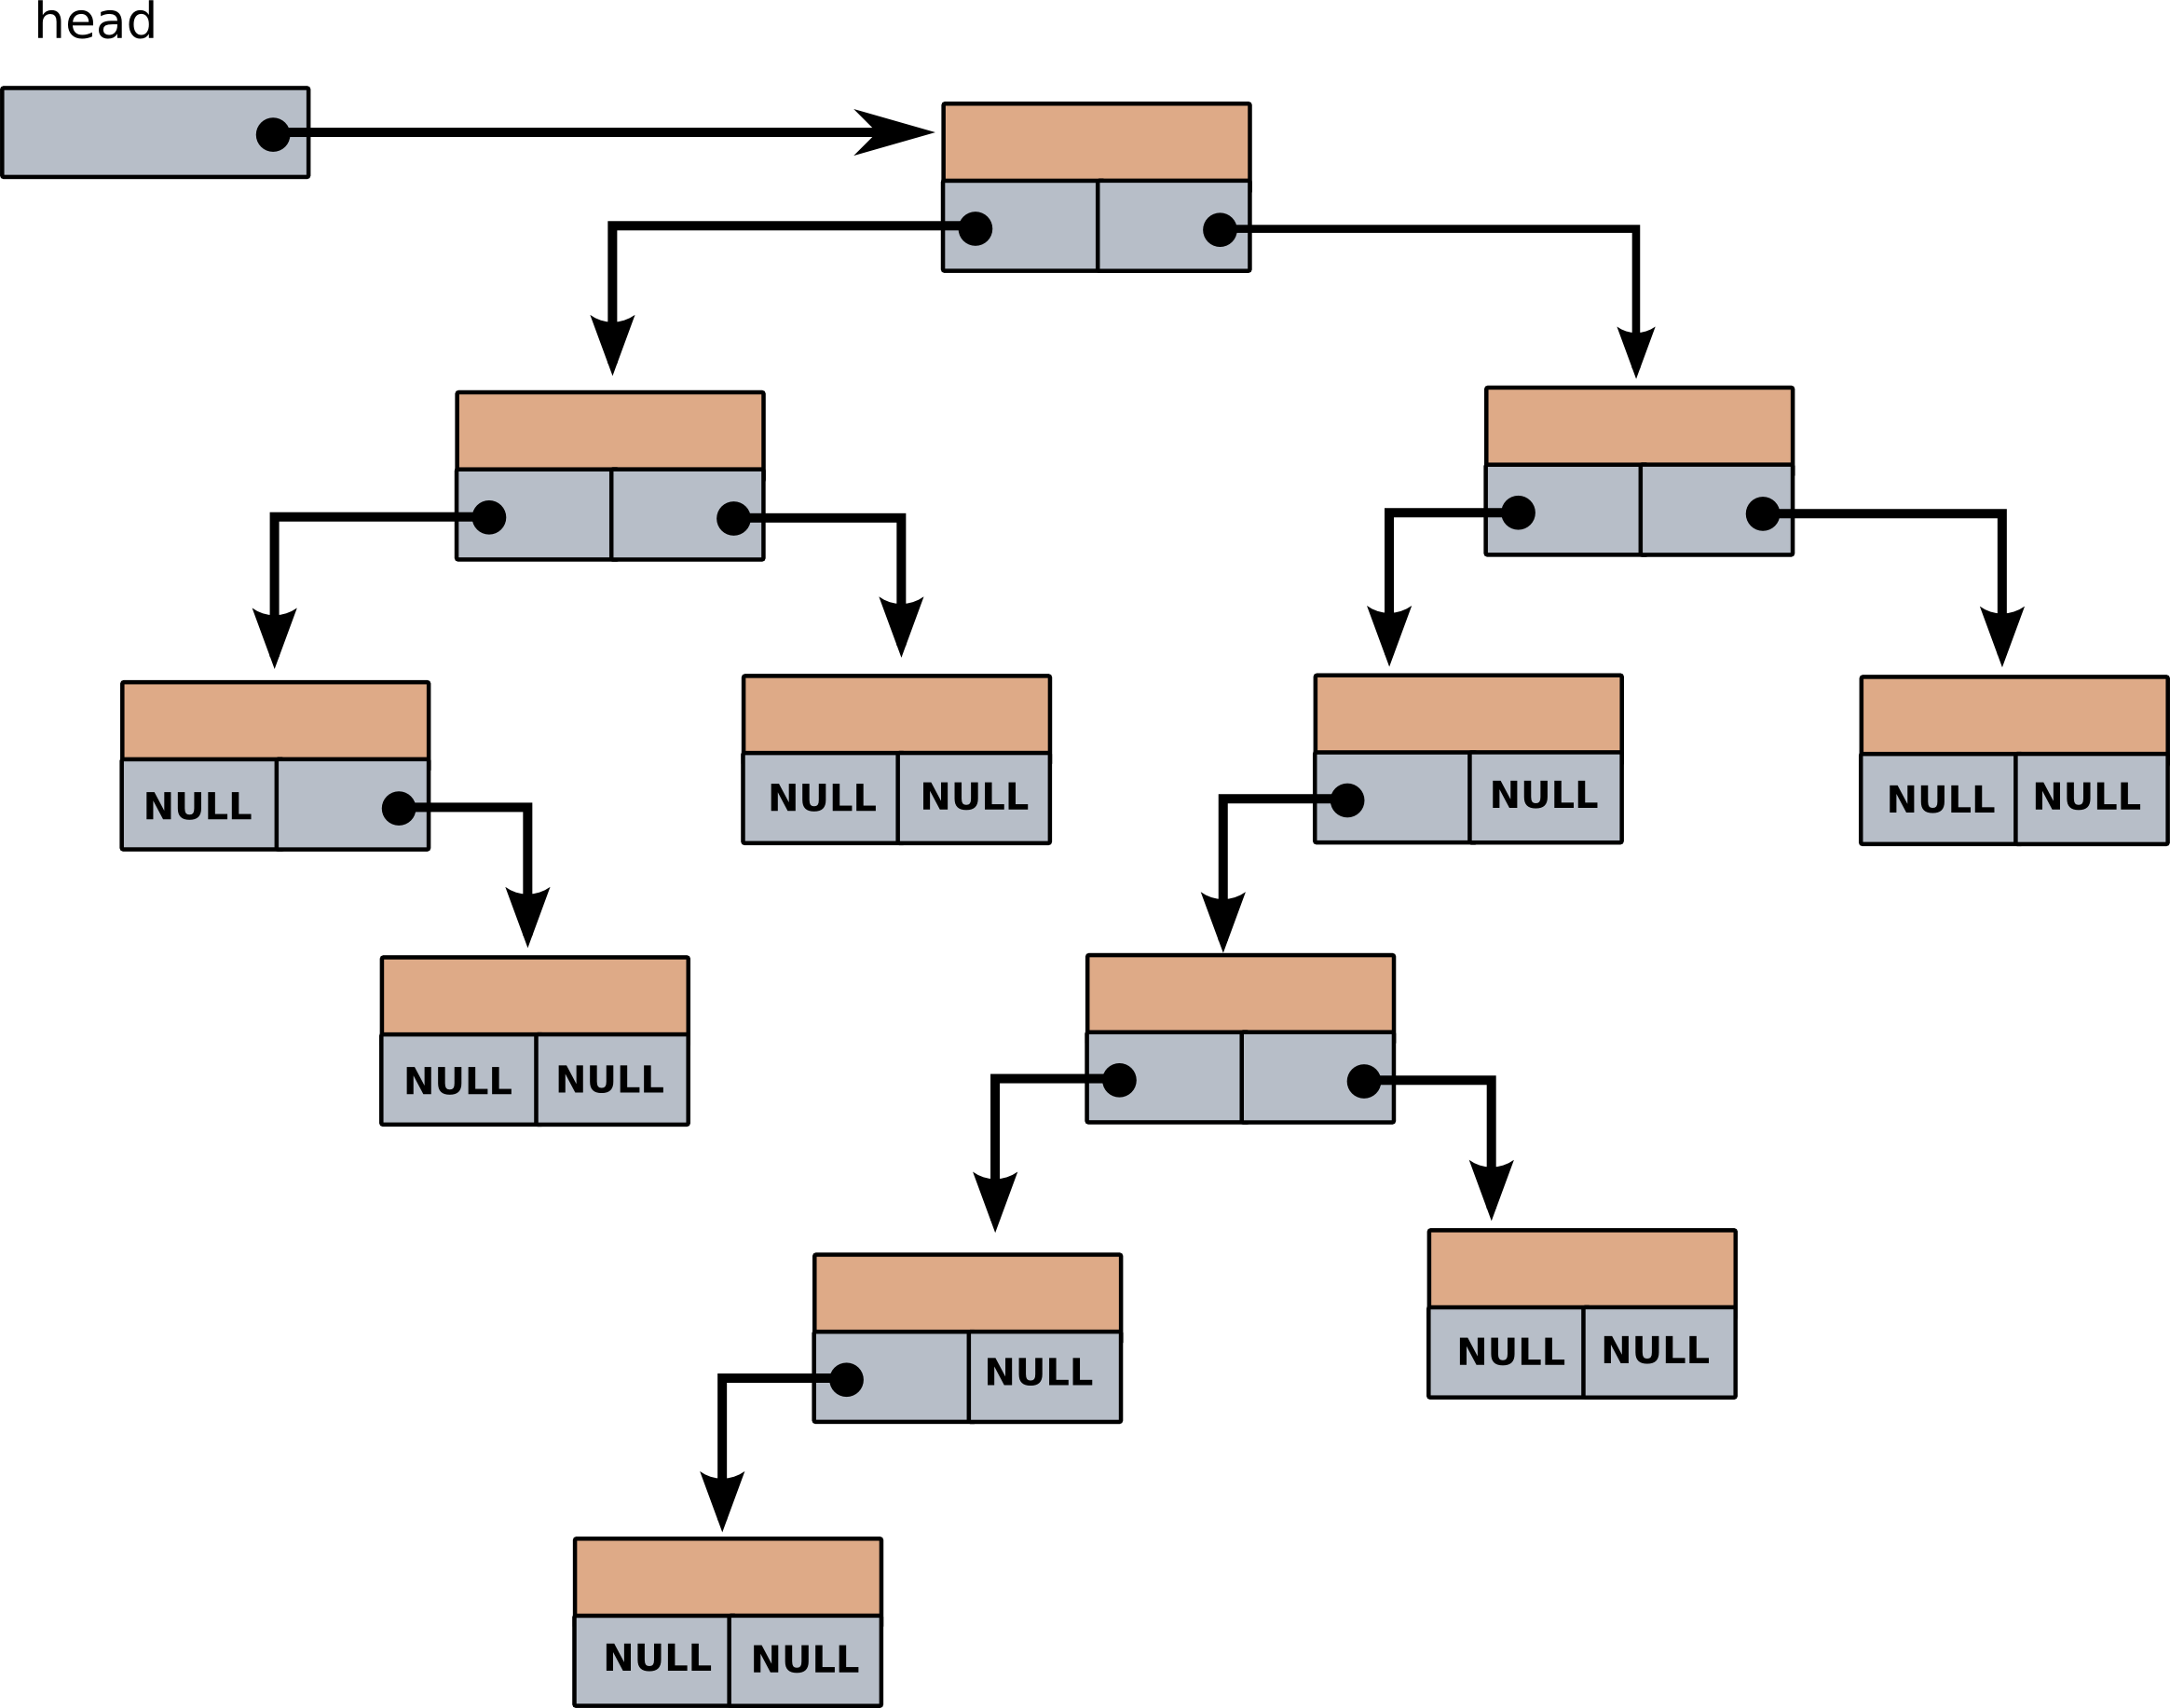
\includegraphics[width=0.75\linewidth]{images/bintree_initial_2.png}
\end{center}
\end{frame}

\begin{frame}[fragile]
\frametitle{Двоичные деревья (обход)}  
\begin{center}
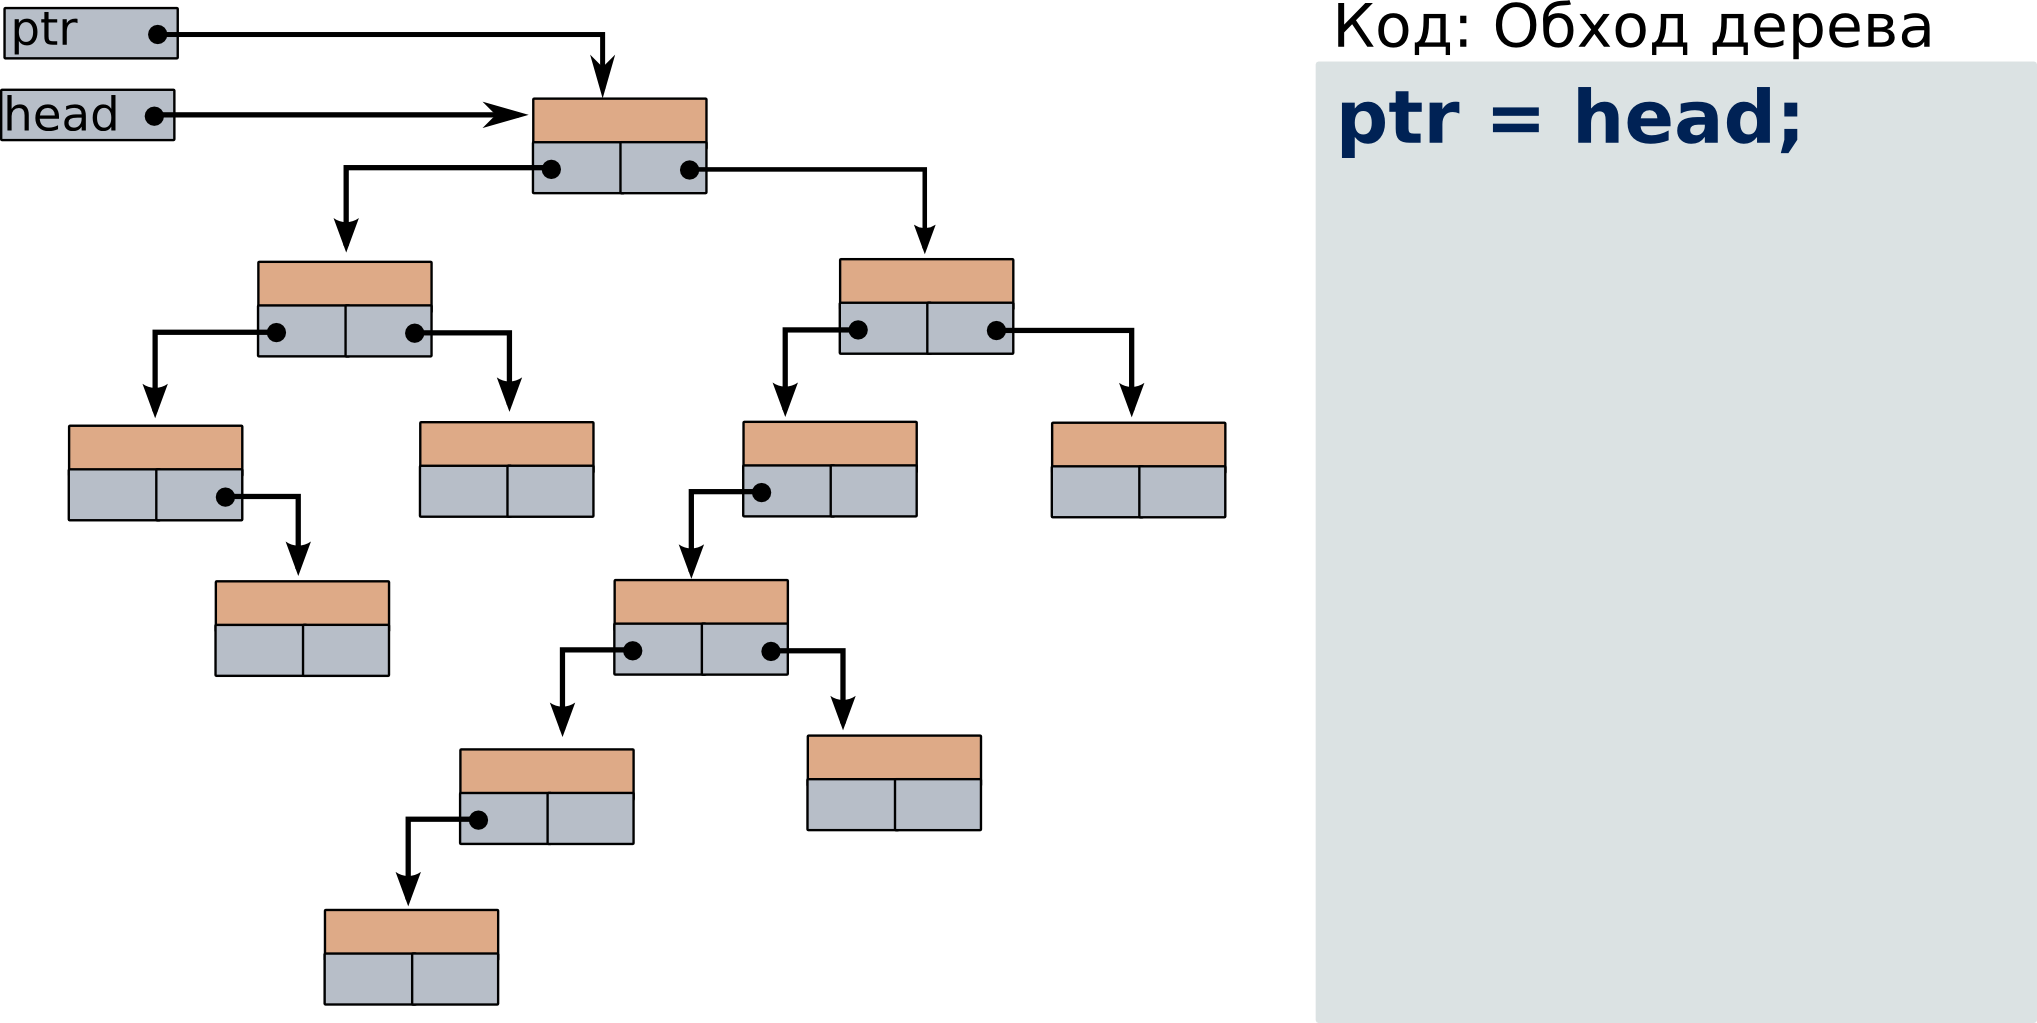
\includegraphics[width=0.99\linewidth]{images/bintree_traversal_1.png}
\end{center}
\end{frame}

\begin{frame}[fragile]
\frametitle{Двоичные деревья (обход)}  
\begin{center}
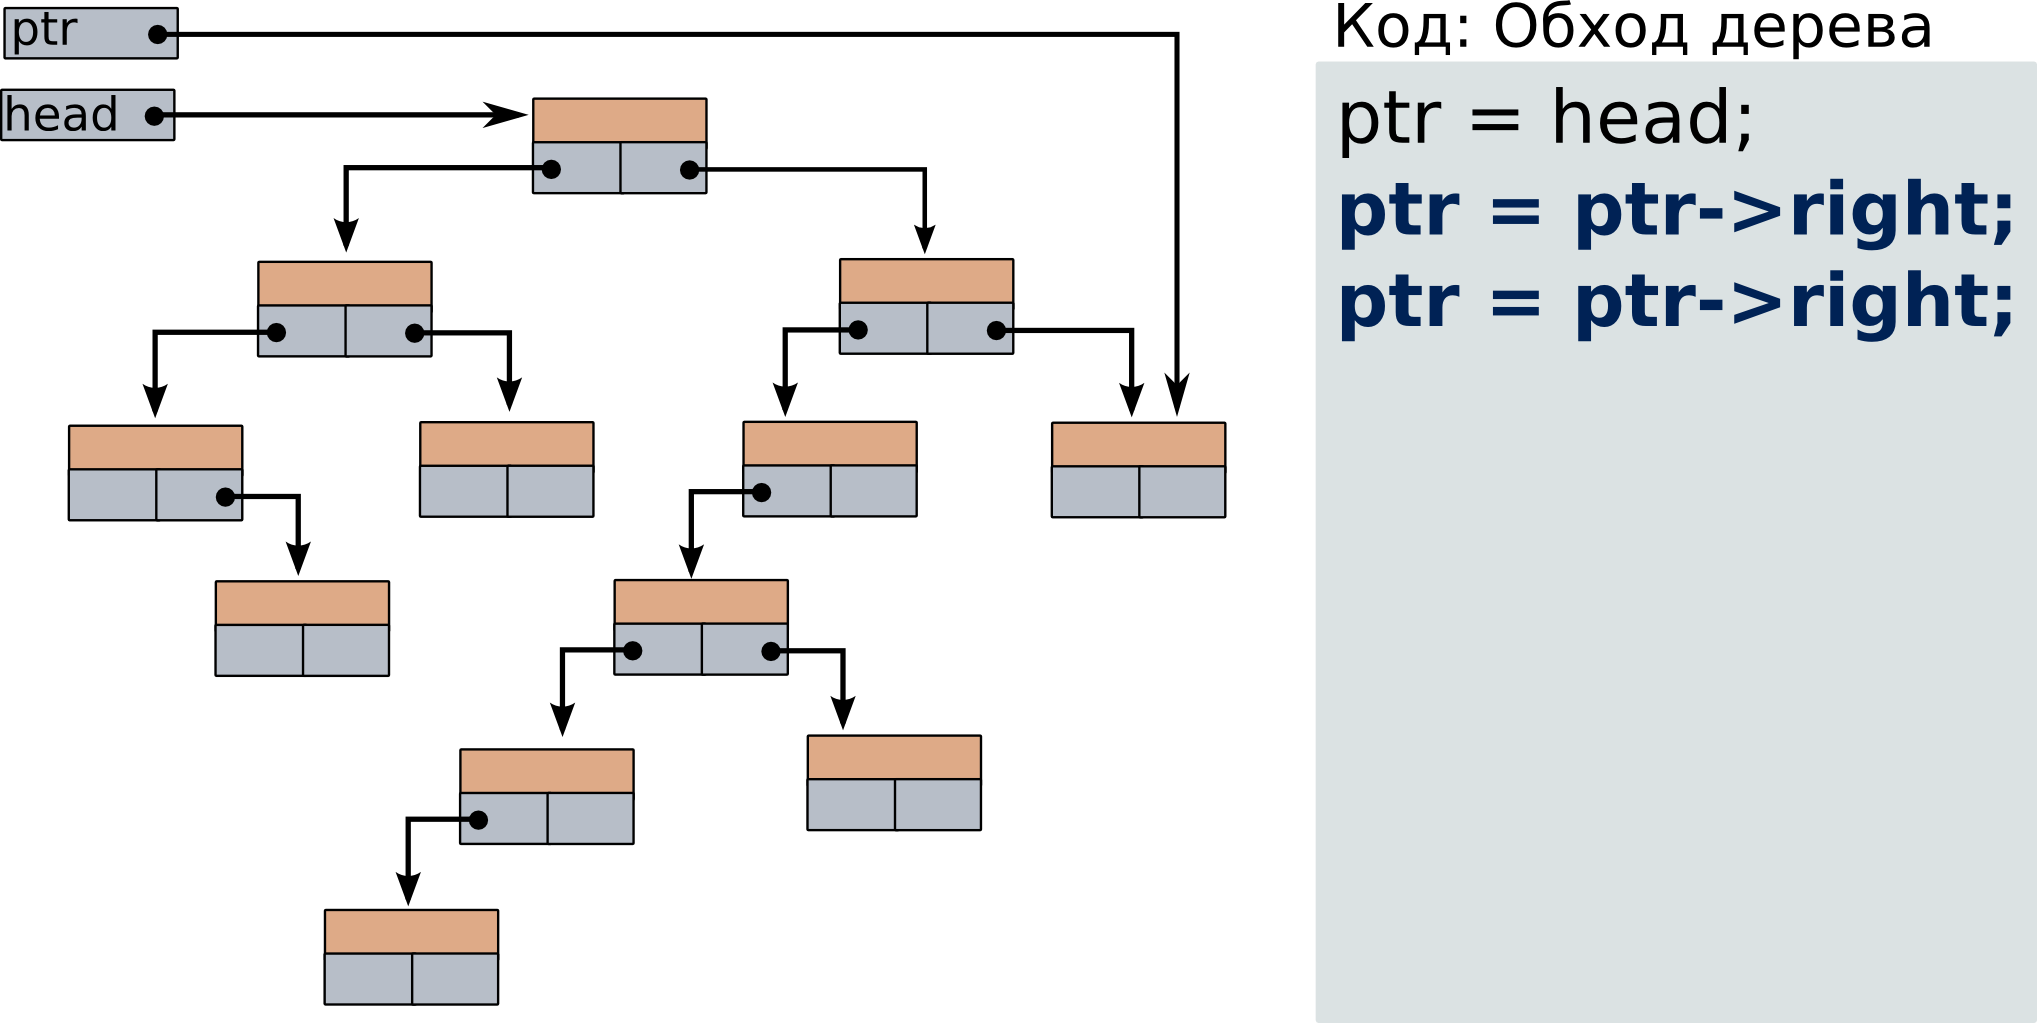
\includegraphics[width=0.99\linewidth]{images/bintree_traversal_2.png}
\end{center}
\end{frame}

\begin{frame}[fragile]
\frametitle{Двоичные деревья (обход)}  
\begin{center}
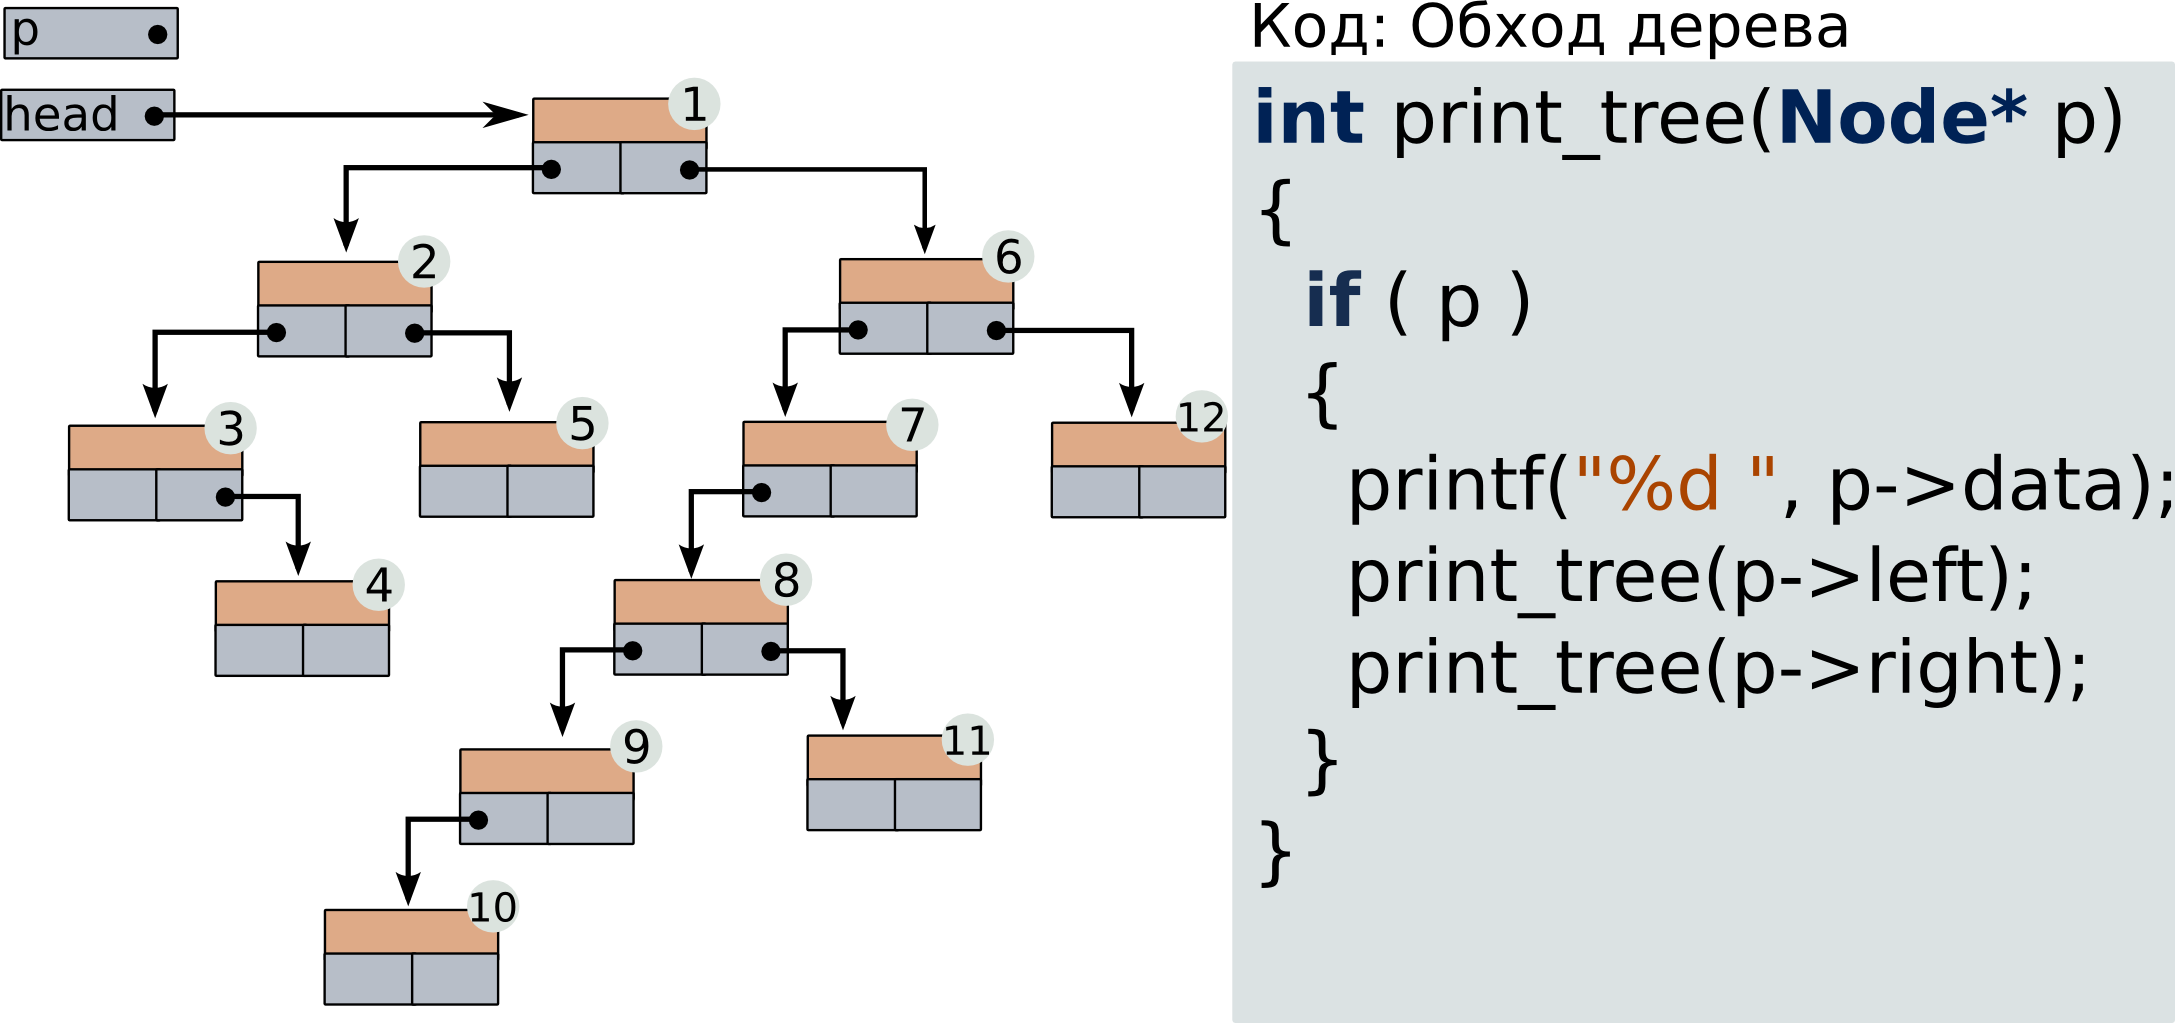
\includegraphics[width=0.99\linewidth]{images/bintree_traversal_3.png}
\end{center}
\end{frame}




\begin{frame}[fragile]
\frametitle{Двоичные деревья поиска} 
\begin{itemize}
\item Двоичные деревья поиска -- это двоичное дерево, обладающее следующим свойством:
\item Пусть $x$ -- произвольная вершина двоичного дерева поиска. Если вершина $y$ находится в левом поддереве
вершины $x$, то $y.data \leq x.data$. Если $y$ находится в правом поддереве вершины $x$, то $y.data \geq x.data$. 
\end{itemize}
\end{frame}

\begin{frame}[fragile]
\frametitle{Двоичные деревья поиска}  
\begin{center}
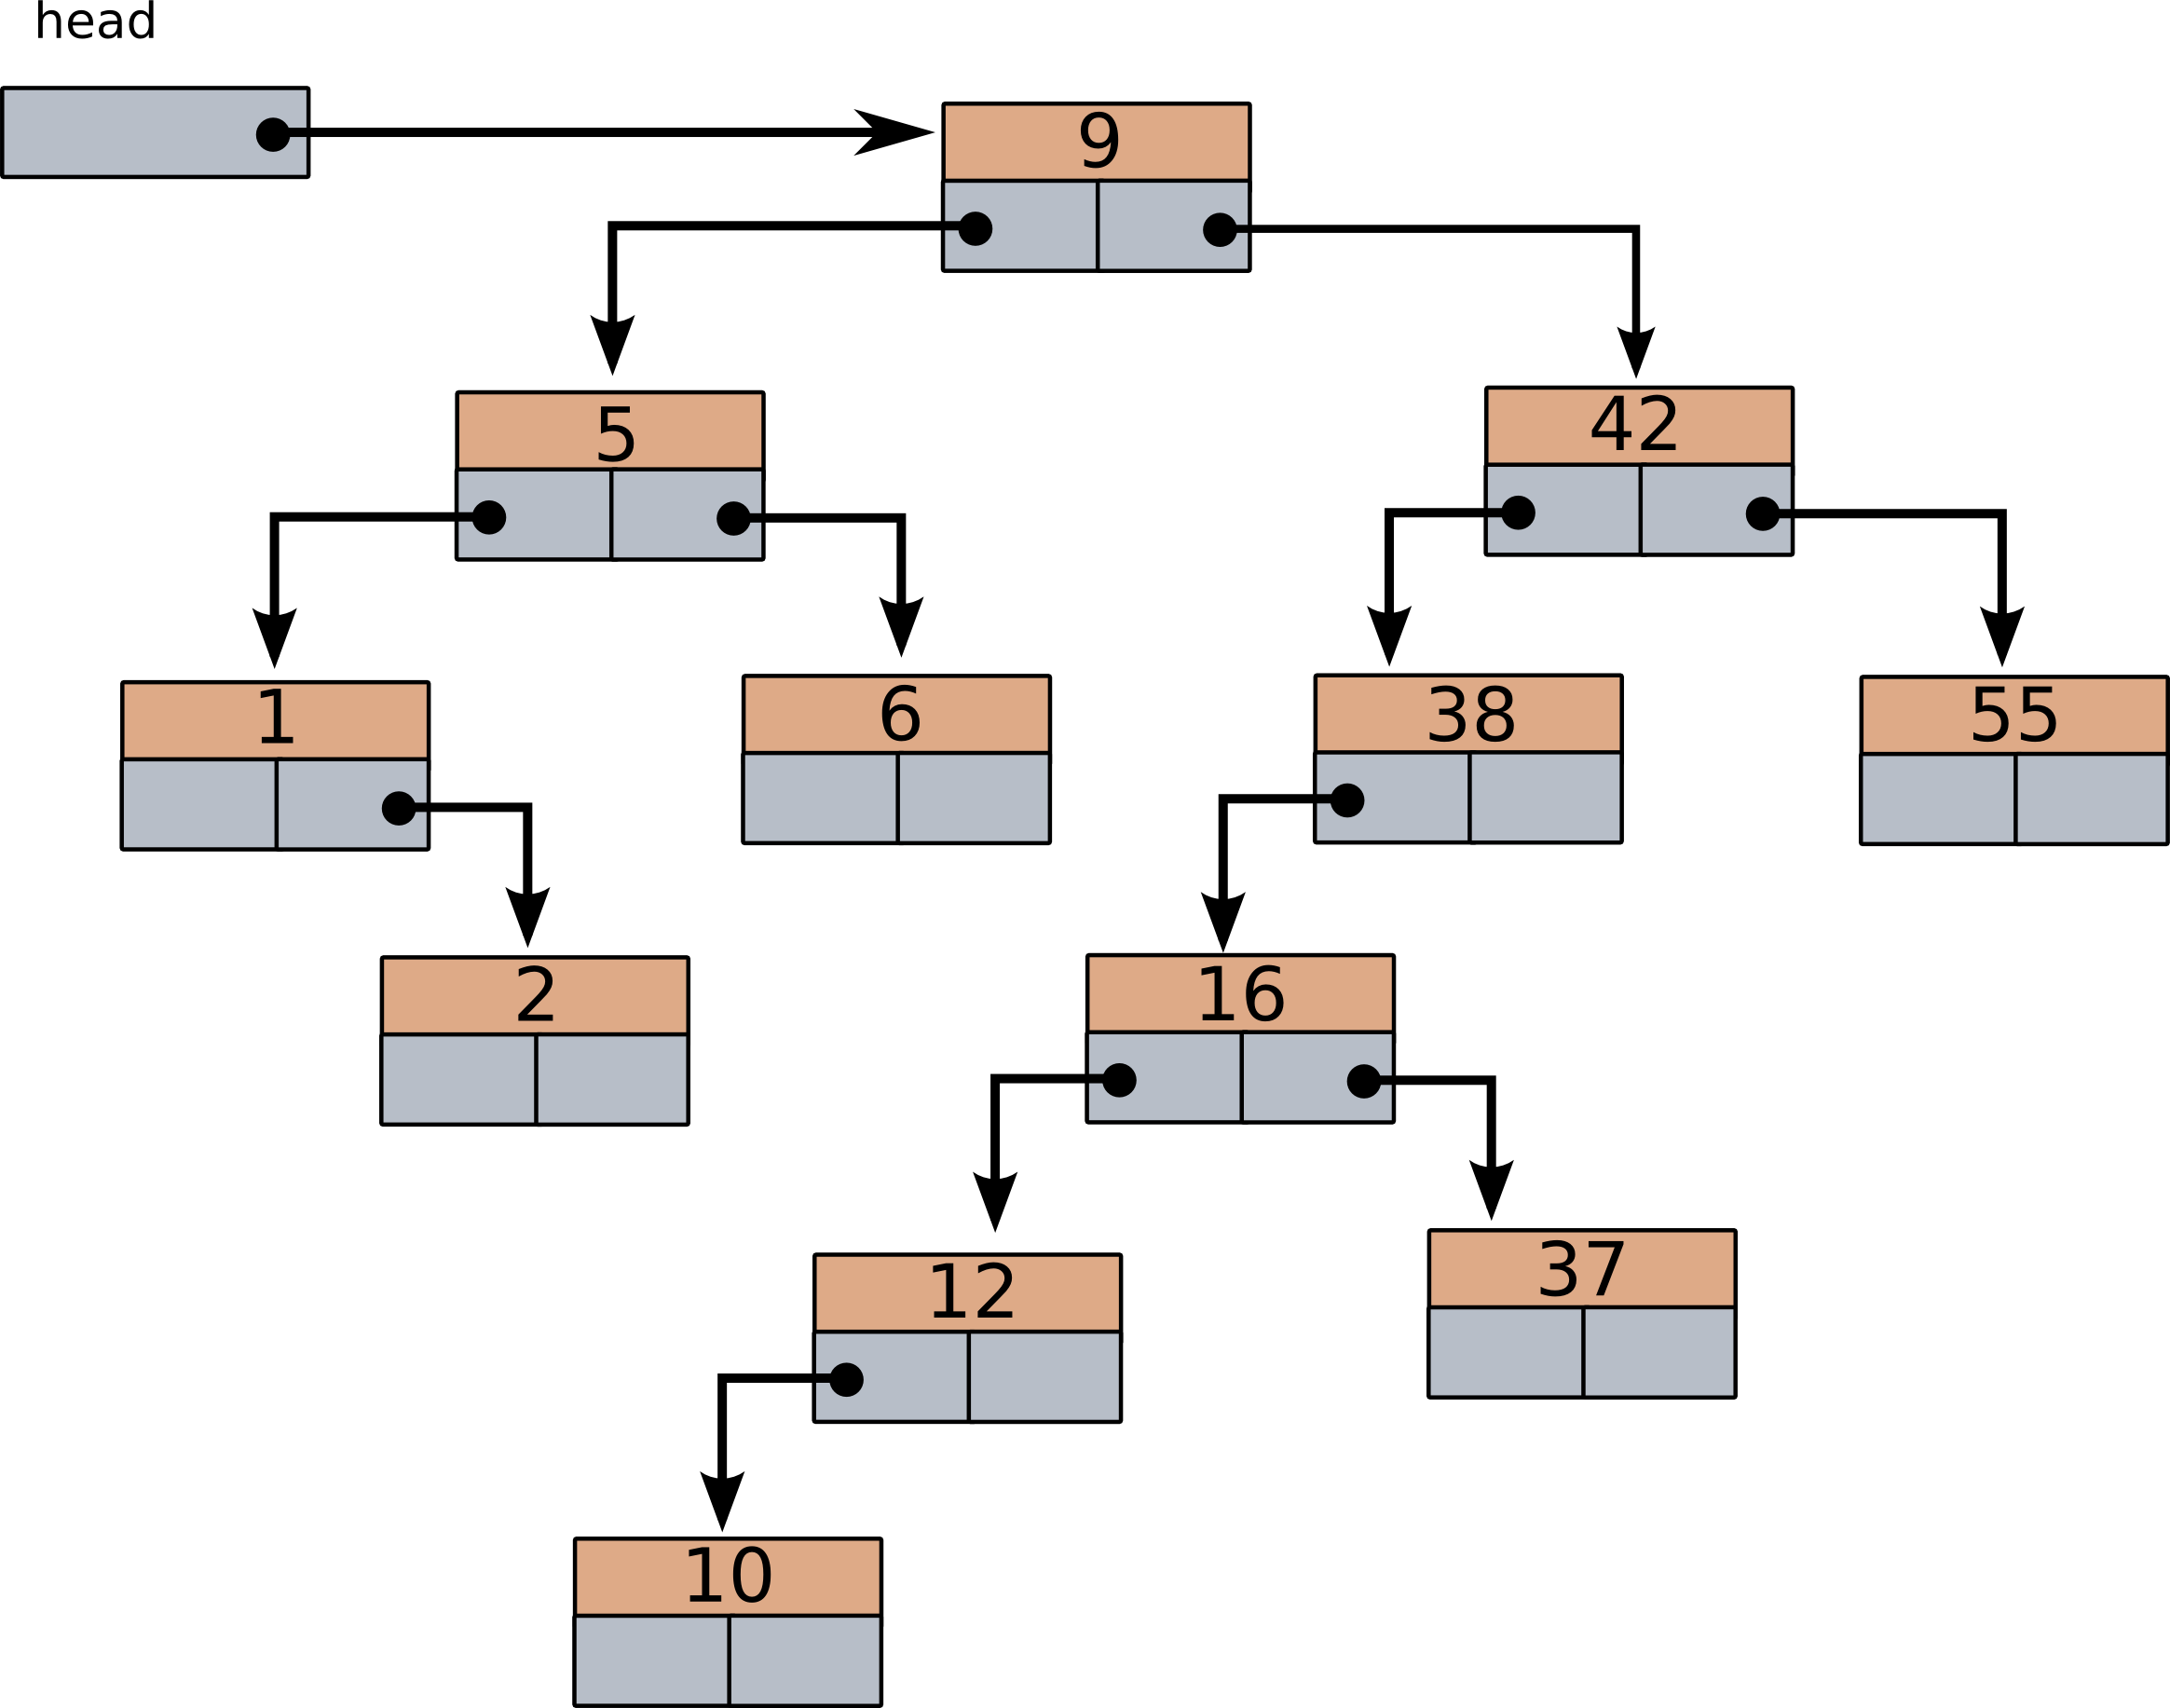
\includegraphics[width=0.75\linewidth]{images/bintree_search_1.png}
\end{center}
\end{frame}



\end{document}